\documentclass[11pt,a4paper]{article}

\usepackage[margin=1in]{geometry}
\usepackage[T1]{fontenc}
\usepackage[utf8]{inputenc}
\usepackage{lmodern}
\usepackage{microtype}
\usepackage{graphicx}
\usepackage{float}
\usepackage{xcolor}
\usepackage{hyperref}
\usepackage{enumitem}
\usepackage{booktabs}
\usepackage{array}
\usepackage{titlesec}
\usepackage{setspace}
\usepackage{fancyhdr}

\definecolor{DormDeskBlue}{HTML}{163A63}
\definecolor{DormDeskSlate}{HTML}{4A5A6A}
\definecolor{DormDeskLight}{HTML}{F4F7FB}
\definecolor{DormDeskAccent}{HTML}{2B5D8A}

\hypersetup{
  colorlinks=true,
  linkcolor=DormDeskBlue,
  urlcolor=DormDeskAccent,
  citecolor=DormDeskBlue,
  pdftitle={DormDesk Project Report},
  pdfauthor={Cloud Backend Architect & Full-Stack Developer}
}

\titleformat{\section}{\Large\bfseries\color{DormDeskBlue}}{\thesection}{0.75em}{}
\titleformat{\subsection}{\large\bfseries\color{DormDeskSlate}}{\thesubsection}{0.75em}{}
\titleformat{\subsubsection}{\normalsize\bfseries\color{DormDeskSlate}}{\thesubsubsection}{0.75em}{}

\pagestyle{fancy}
\fancyhf{}
\lhead{\color{DormDeskSlate}DormDesk Project Report}
\rhead{\color{DormDeskSlate}\thepage}
\setlength{\headheight}{23.2pt}
\renewcommand{\headrulewidth}{0.4pt}
\renewcommand{\headrule}{\hbox to\headwidth{\color{DormDeskSlate}\leaders\hrule height \headrulewidth\hfill}}

\setstretch{1.12}
\setlist[itemize]{leftmargin=1.4em, itemsep=0.3em, topsep=0.3em}
\setlist[enumerate]{leftmargin=1.6em, itemsep=0.3em, topsep=0.3em}

\begin{document}

\begin{titlepage}
  \centering
  \vspace*{1.5cm}
  {\Huge\bfseries\color{DormDeskBlue} DormDesk\par}
  \vspace{0.35cm}
  {\Large\color{DormDeskSlate} Role-Based Hostel Complaint Management System\par}
  \vspace{1.4cm}
  {\large\color{DormDeskSlate}Project Documentation Report\par}
  \vspace{1.8cm}

  \begin{table}[H]
    \centering
    \renewcommand{\arraystretch}{1.35}
    \begin{tabular}{>{\bfseries}p{0.28\textwidth} p{0.58\textwidth}}
      \toprule
      Project Name & DormDesk \\
      Subtitle & Role-Based Hostel Complaint Management System \\
      Role & Cloud Backend Architect \& Full-Stack Developer \\
      Tech Stack & AWS (Cognito, Lambda, EC2), Node.js, Express, React, Tailwind CSS, Docker, Nginx, PostgreSQL/MongoDB \\
      \bottomrule
    \end{tabular}
  \end{table}

  \vfill
  {\large\color{DormDeskSlate}Generated for professional project documentation and presentation\par}
\end{titlepage}

\tableofcontents
\newpage

\section{Problem Statement \& Motivation}
Traditional hostel complaint handling is often fragmented. Students rely on physical registers, informal WhatsApp groups, or handwritten slips to report issues. Those channels create a predictable set of problems: complaints get lost, status updates are inconsistent, ownership is unclear, and there is little accountability for maintenance teams or hostel administrators.

DormDesk addresses that gap by providing a centralized, transparent, full-stack complaint lifecycle platform. Every complaint moves through a controlled workflow from submission to resolution, with access restricted by role and every administrative action recorded for traceability. The result is a system that reduces friction for students, improves visibility for hostel staff, and creates a dependable audit trail for management.

\section{System Architecture \& Core Features}
DormDesk is designed as a role-aware platform with a clear separation between the user interface, API layer, and cloud infrastructure. It combines a React-based frontend, a Node.js and Express backend, and deployment components suited for containerized cloud hosting.

\subsection{Role-Based Access Control (RBAC)}
Access is divided across multiple user categories to keep the system secure and focused:
\begin{itemize}
  \item \textbf{Students} can register, submit complaints, and track their own tickets.
  \item \textbf{Super Admins} can view and manage all complaints across categories.
  \item \textbf{Department-Specific Admins} can work only within their assigned domains, including Food, Water, Electrical, Cleaning, and Room.
\end{itemize}
This model prevents unauthorized access while keeping each role’s interface simple and relevant.

\subsection{Lifecycle Management}
Each complaint moves through a four-stage visual lifecycle:
\begin{center}
\fbox{\colorbox{DormDeskLight}{\parbox{0.9\textwidth}{\centering Received $\rightarrow$ Acknowledged $\rightarrow$ In Progress $\rightarrow$ Resolved}}}
\end{center}
This stage model makes progress easy to understand at a glance and supports structured escalation and closure.

\subsection{Accountability \& Auditing}
DormDesk records every meaningful administrative transition in an audit log. That includes the stage change, the person who performed it, the note attached to the action, and the timestamp. This creates visibility into what happened, when it happened, and who made the decision.

\subsection{Cloud Infrastructure}
The deployment model uses Docker containers behind an Nginx reverse proxy, with AWS services supporting authentication and automation. Cognito handles identity and group-based access, while Lambda is available for background triggers and future workflow extensions. This architecture is production-oriented and can be adapted to either single-host deployment or cloud-hosted scaling patterns.

\section{Visual Walkthrough \& Implementation}
The following screenshots document the primary user journey and the administrative control surfaces of the system.

\subsection{Authentication Interface}
Figure~\ref{fig:login} shows the clean login screen and the local test credential panel. This view supports fast role switching during development and demonstrates the authentication entry point for students and administrators.

\begin{figure}[H]
  \centering
  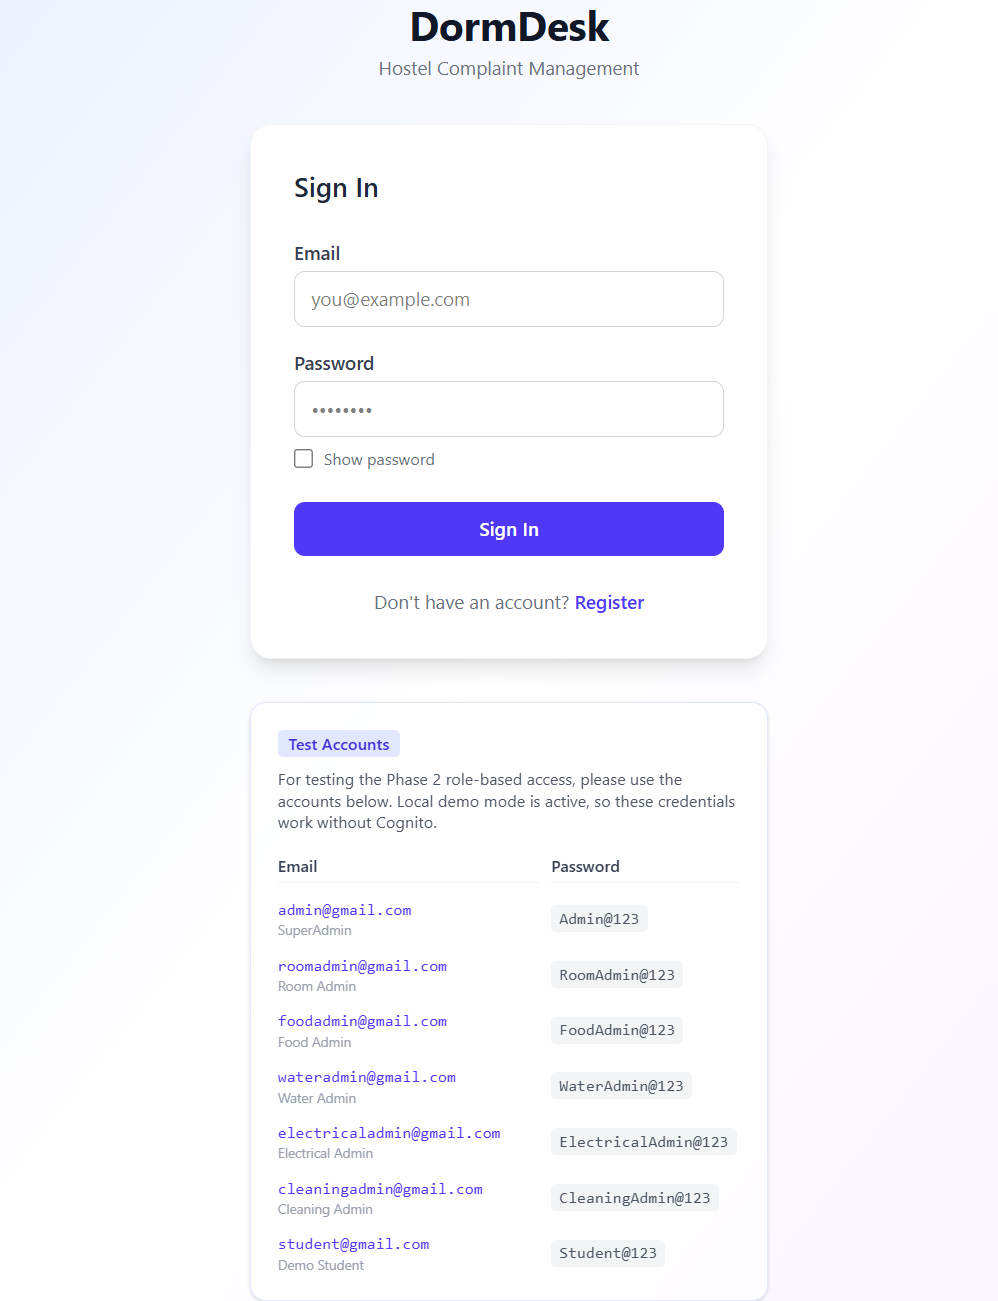
\includegraphics[width=0.85\textwidth]{screenshots/01-login-page.png}
  \caption{Authentication interface with local test credentials for role-based testing.}
  \label{fig:login}
\end{figure}

\subsection{Student Complaint Dashboard}
Figure~\ref{fig:student} highlights the student workflow. The complaint form captures category, description, and priority, while the complaint list shows real-time visual progress for submitted tickets.

\begin{figure}[H]
  \centering
  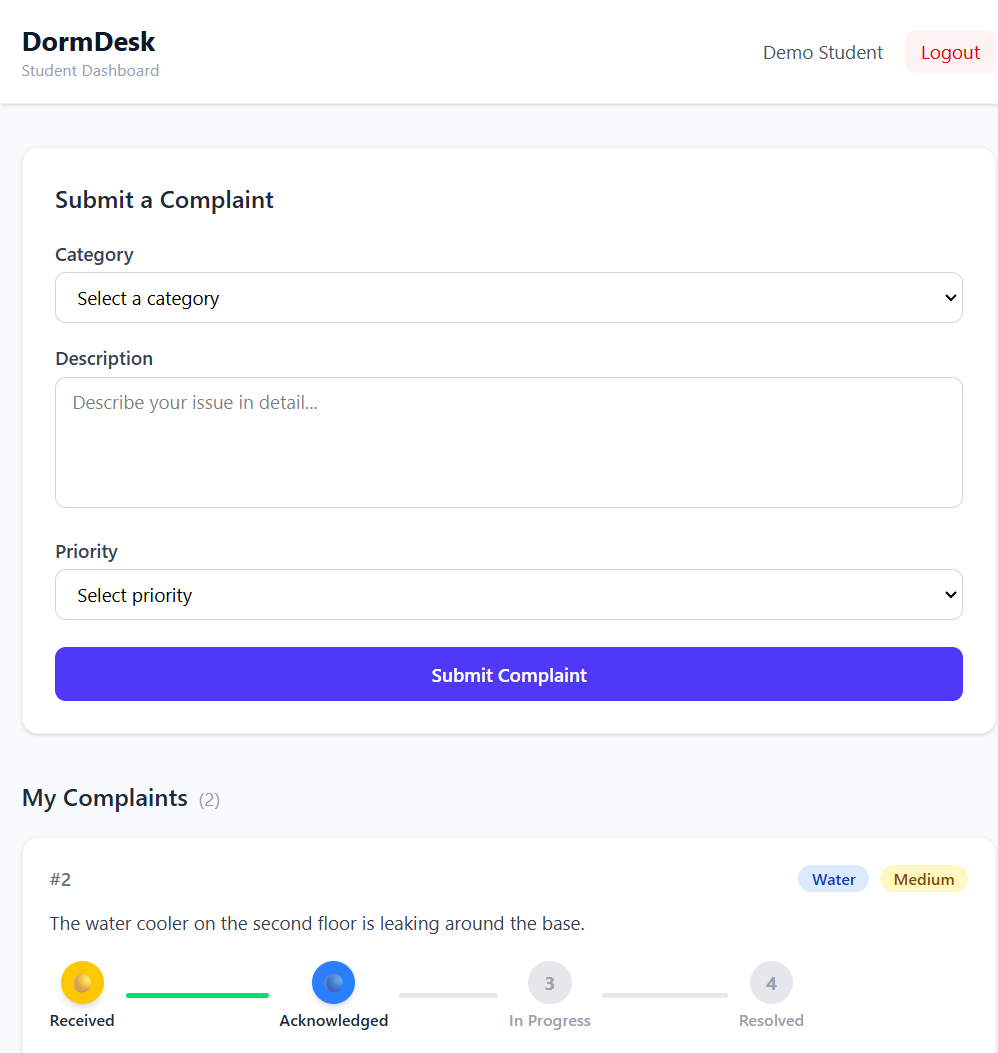
\includegraphics[width=0.85\textwidth]{screenshots/02-student-dashboard.png}
  \caption{Student dashboard with complaint submission and live status tracking.}
  \label{fig:student}
\end{figure}

\subsection{Admin Management Console}
Figure~\ref{fig:admin} shows the admin control panel. It provides granular filters by category, priority, and stage, along with action buttons that allow administrators to advance or revert complaints through the workflow.

\begin{figure}[H]
  \centering
  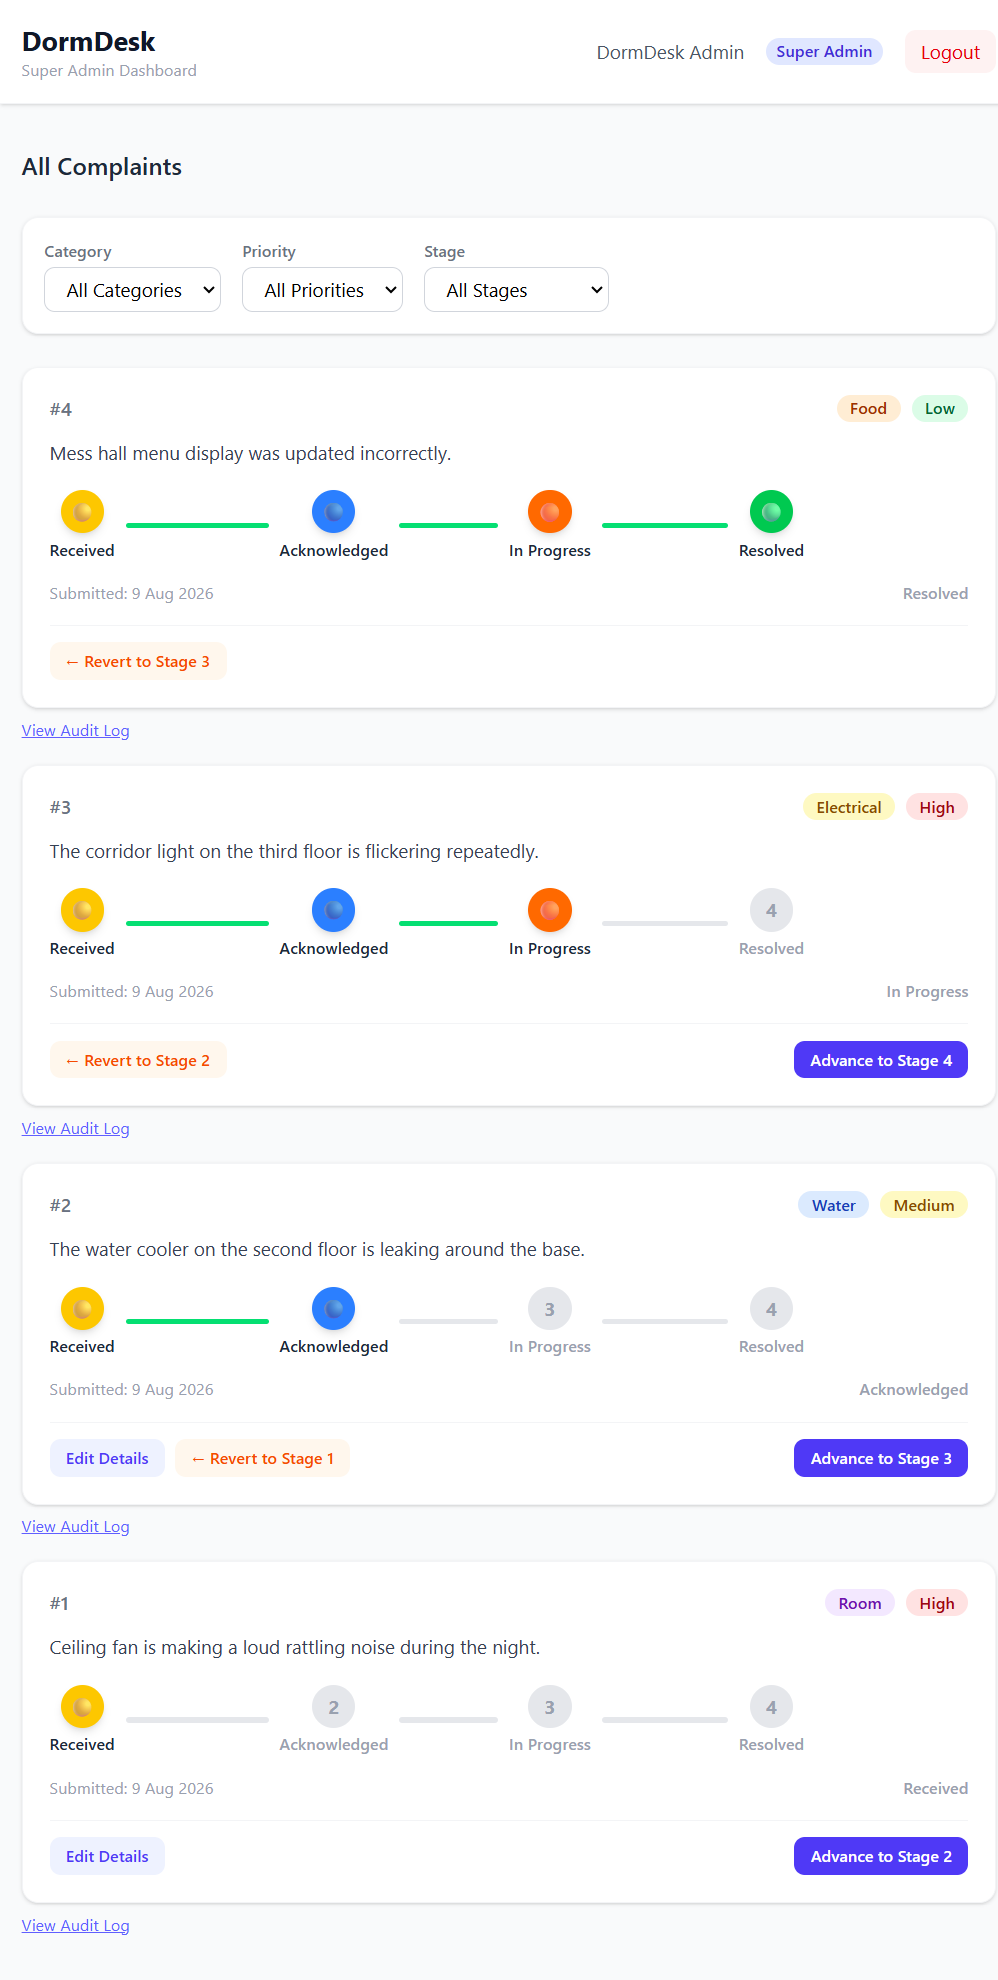
\includegraphics[width=0.85\textwidth]{screenshots/03-admin-dashboard.png}
  \caption{Admin dashboard with filters and workflow control actions.}
  \label{fig:admin}
\end{figure}

\subsection{Audit Log Transparency Layer}
Figure~\ref{fig:audit} illustrates the accountability layer. The modal lists timestamped history entries for each administrative change, making the lifecycle of a complaint fully traceable.

\begin{figure}[H]
  \centering
  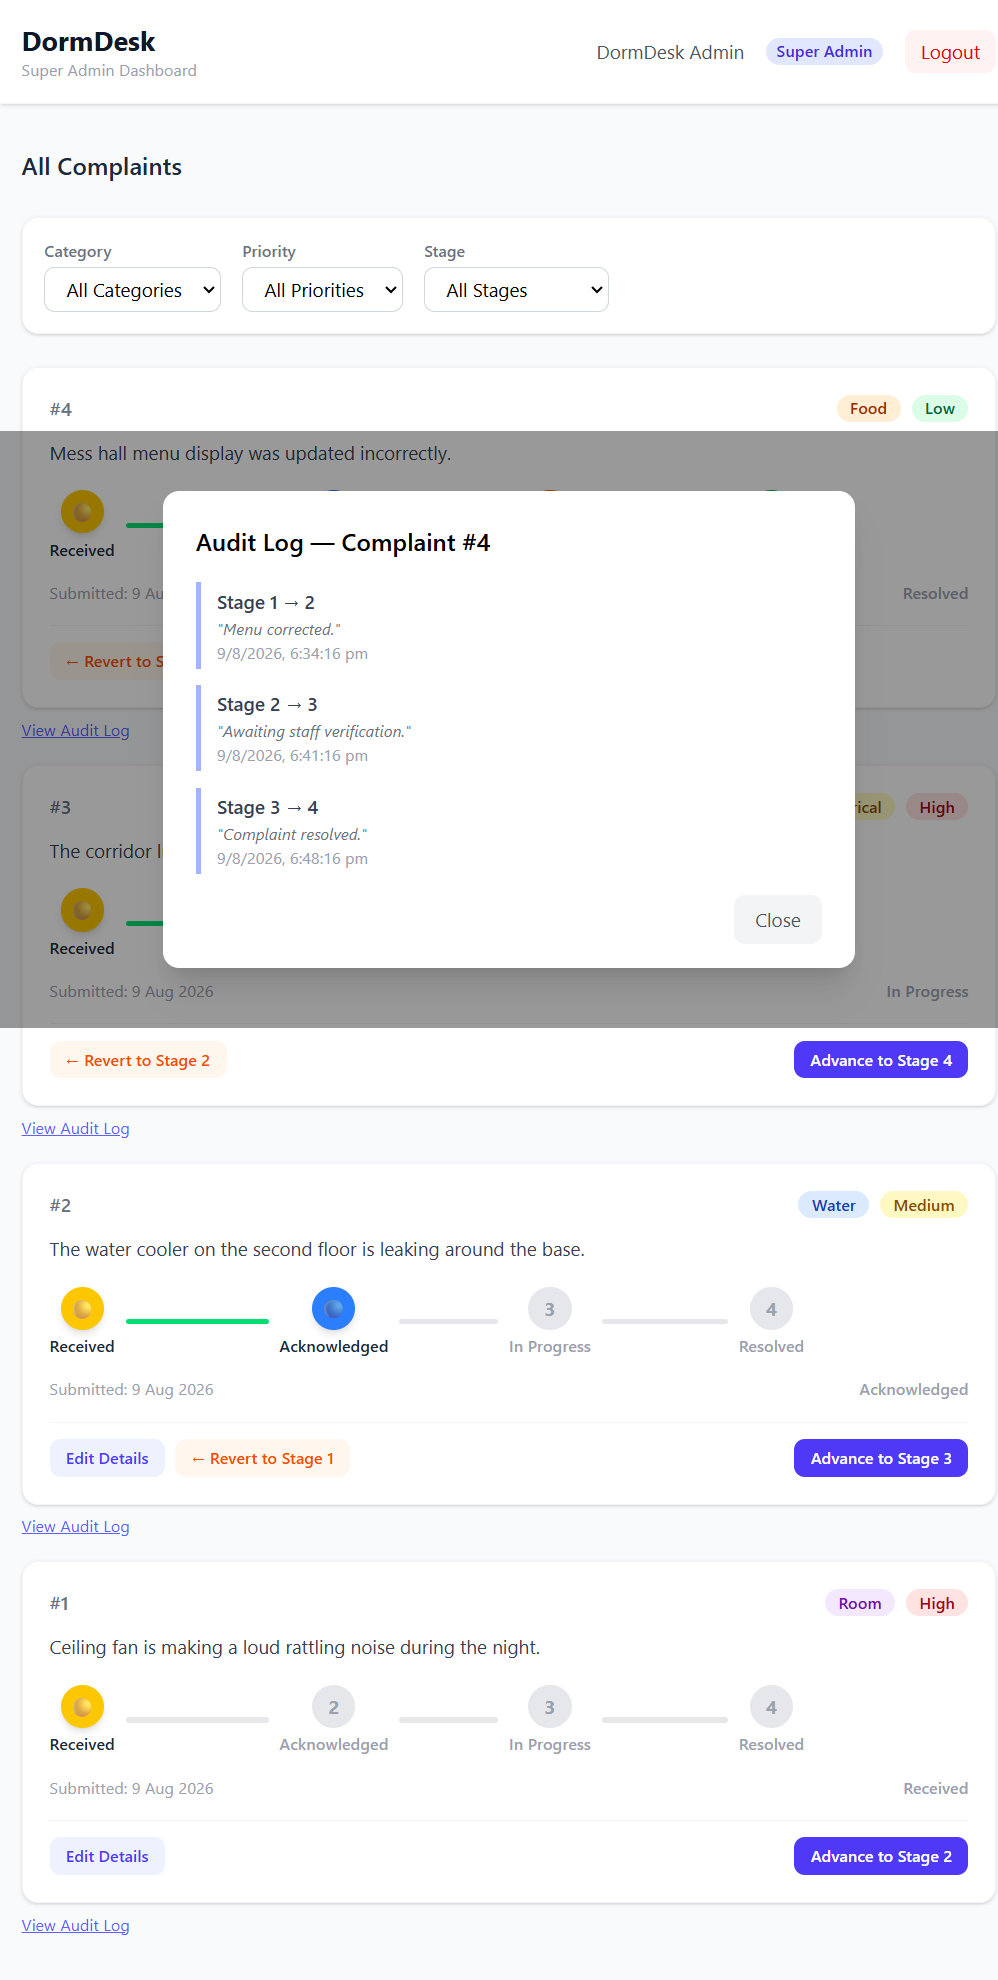
\includegraphics[width=0.85\textwidth]{screenshots/04-audit-log-modal.png}
  \caption{Audit log modal showing the full status transition history for a complaint.}
  \label{fig:audit}
\end{figure}

\section{Conclusion \& Business Value}
DormDesk eliminates the communication gaps that commonly affect institutional housing operations. Instead of relying on informal updates or paper-based processes, the platform centralizes complaints, assigns clear role boundaries, and preserves a complete record of every change.

From a technical perspective, the project demonstrates a production-ready cloud architecture with containerization, reverse proxying, role-based authentication, and an auditable workflow model. From a business perspective, it improves maintenance responsiveness, reduces confusion, and gives hostel management a reliable operational record that can be used for reporting, accountability, and service improvement.

\vspace{0.5cm}
\noindent\textbf{Project Outcome:} DormDesk provides a scalable foundation for digital hostel operations and can be extended with notifications, analytics, automated escalation, and deeper cloud integrations.

\end{document}
